\documentclass[xcolor=table,aspectratio=169,dvipsnames,english]{beamer}
\usepackage{bm}
\usepackage[utf8]{inputenc}
\usepackage{color}

\usepackage[british]{babel} % decent hyphenation, avoiding e.g. anal-ysis
\usepackage[iso]{isodate}
\usepackage{sansmath}
\usepackage{booktabs}
\usepackage{graphicx}
\usepackage{graphviz}
\usepackage{makecell}
\usepackage{minted}
\usepackage{multicol}
\usepackage{siunitx}
\usepackage{subcaption}
\usepackage[section]{placeins}

% Needs to be loaded after hyperref
\usepackage{cleveref}

% PythonTeX
\usepackage[autoprint=false, gobble=auto, keeptemps=all, pyfuture=all]{pythontex} % create figures on-line directly from python!
\usepackage{pgf}
%\input{/usr/share/repsep/functions.py}
\input{functions.py}
\begin{pythontexcustomcode}[begin]{py}
pytex.add_dependencies(
	'lib/utils.py',
	'lib/categorical.py',
	'data/JogB.tsv'
	)
\end{pythontexcustomcode}
% Single-session PythonTeX codeblocks
\newcounter{pysessioncounter}
\newcommand{\sessionpy}{%
          \edef\sessionpysession{session\arabic{pysessioncounter}}%
            \stepcounter{pysessioncounter}%
              \expandafter\py\expandafter[\sessionpysession]}

% SIunitx customizations detect-all will use the current font for typesetting
\sisetup{per-mode=symbol, detect-all, range-units = single}
\newcommand\SIci[5]{\SI{#1}{#2}, {#3}CI: \SIrange{#4}{#5}{#2}}

% Fix for matplotlib PGF wonkiness which isn't interpreted correctly by pdflatex
\DeclareUnicodeCharacter{2212}{-}


%\hypersetup{
%    colorlinks=true,
%    urlcolor=cyan
%}

%BIBLIOGRAPHY
% see https://mirror.foobar.to/CTAN/macros/latex/contrib/biblatex/doc/biblatex.pdf for available styles
\usepackage[backend=bibtex,style=numeric,natbib=true]{biblatex}
\addbibresource{bib.bib}
\addbibresource{old_bib.bib}

% Article-specific configuration
\begin{pythontexcustomcode}[begin]{py}
DOC_STYLE="slides/main.conf"
pytex.add_dependencies(
	DOC_STYLE,
	'slides/1col.conf',
	)
\end{pythontexcustomcode}

% Custom beamer styling and colors
\setbeamersize{text margin left=0.8em,text margin right=0.8em}
\setbeamertemplate{bibliography item}{\insertbiblabel}

\usecolortheme[RGB={199,199,199}]{structure}
\usetheme{Dresden}

\captionsetup[figure]{labelformat=empty}

\definecolor{dy}{RGB}{202,202,0}
\definecolor{rsblue}{HTML}{00a3cc}
\definecolor{mg}{gray}{0.30}
\definecolor{lg}{gray}{0.60}
\definecolor{vlg}{gray}{0.78}
\definecolor{tlg}{gray}{0.88}

\setbeamercolor{caption name}{fg=lg}
\setbeamercolor{caption}{fg=lg}
\setbeamercolor{author}{fg=lg}
\setbeamercolor{institute}{fg=lg}
\setbeamercolor{date}{fg=lg}
\setbeamercolor{title}{fg=mg}
\setbeamertemplate{caption}{\centering\insertcaption\par}
\setbeamertemplate{navigation symbols}{}

% Navigation symbols are too far down by default
% To further adjust edit the pt numbers before and after `\insertnavigation`
\makeatletter
\defbeamertemplate*{headline}{my miniframes theme}
{%
        \begin{beamercolorbox}[colsep=1.5pt]{upper separation line head}
        \end{beamercolorbox}
        \begin{beamercolorbox}{section in head/foot}
                \vskip1pt\insertnavigation{\paperwidth}\vskip3pt
        \end{beamercolorbox}%
        \ifbeamer@theme@subsection%
                \begin{beamercolorbox}[colsep=1.5pt]{middle separation line head}
                \end{beamercolorbox}
                \begin{beamercolorbox}[ht=2.5ex,dp=1.125ex,%
                        leftskip=.3cm,rightskip=.3cm plus1fil]{subsection in head/foot}
                        \usebeamerfont{subsection in head/foot}\insertsubsectionhead
                \end{beamercolorbox}%
        \fi%
        \begin{beamercolorbox}[colsep=1.5pt]{lower separation line head}
        \end{beamercolorbox}
}
\makeatother


\title{Multimodal Generative Learning on the MIMIC-CXR Database}
\subtitle{A presentation of my semester project}
\author{Hendrik Klug}
\institute{Institute for Electrical Engineering, ETH}
\begin{document}
    \begin{frame}
        \titlepage
    \end{frame}


    \section{Introduction}

    \begin{frame}
        In this work, we applied a method for \textbf{self-supervised}, \textbf{multimodal} and \textbf{generative} training proposed by Sutter et al. \footcite{thomas_multimodal} on medical data from the MIMIC-CXR Database \footcite{johnson2019mimic}.
    \end{frame}

    \subsection{Multimodal, Unsupervised, Generative models}

    \begin{frame}{Self-supervised, multimodal, generative learning?}
        \resizebox{\textwidth}{!}{%
            \begin{tikzpicture}[modalities/.style={rectangle, draw=green!60, fill=green!5, very thick, minimum size=5mm},model/.style={rectangle, draw=red!60, fill=red!5, very thick, minimum size=20mm},lr/.style={ellipse, draw=blue!60, fill=blue!5, very thick, minimum height=5mm,  minimum width=10mm}]
                \node[modalities] (input_text) {Text};
                \node[modalities, below of=input_text] (input_F) {F-Img};
                \node[modalities, below of=input_F] (input_L) {L-Img};
                \node[model, right of=input_F, xshift=2cm] (encoder) {Encoder};
                \node[lr, right of=encoder, xshift=3cm, align=center] (lr) {Latent\\ Representation  \footnote{Assumed to be Gaussian distributed}};
                \node[model, right of=lr, xshift=3cm] (decoder) {Decoder};
                \node[modalities, right of=decoder, xshift=2cm] (out_F) {F-Img};
                \node[modalities, below of=out_F] (out_L) {L-Img};
                \node[modalities, above of=out_F] (out_text) {Text};
                \draw[->] (input_text) -- (encoder);
                \draw[->] (input_F) -- (encoder);
                \draw[->] (input_L) -- (encoder);
                \draw[->] (encoder) -- (lr);
                \draw[->] (lr) -- (decoder);
                \draw[->] (decoder) -- (out_F);
                \draw[->] (decoder) -- (out_text);
                \draw[->] (decoder) -- (out_L);
            \end{tikzpicture}}
    \end{frame}

    \begin{frame}{Multimodal, Unsupervised Generative Learning On Medical Data}
        \large{The advantages:}
        \pause
        \begin{itemize}
            \item No need for labeled data
        \end{itemize}
    \end{frame}

    \begin{frame}{No need for labeled data}
        \begin{itemize}
            \item Model is trained to reconstruct the input image $\rightarrow$ no need for labels
            \item Big advantage over other methods:
            \begin{itemize}
                \item In the medical domain, labeling data requires manual expert input
                \item Labeled medical data is only a small subset of all the medical data available
            \end{itemize}
        \end{itemize}
    \end{frame}



    \begin{frame}{Multimodal, Unsupervised Generative Learning On Medical Data}
        \large{The advantages:}
        \begin{itemize}
            \item No need for labeled data
            \item Can extract features and generate from multiple modalities that exist in the medical domain:
            \pause
            \begin{itemize}
                \item Radiographs from multiple angles or different imaging technologies
                \item Text reports
                \item Electronic health records
            \end{itemize}
            \pause
            \item Can \textbf{generate} \textit{coherent} samples
            \pause
            \item Learned latent representation can be used for \textbf{classification}
            \begin{itemize}
                \item Semantically close samples will be grouped together in the learned latent representation.
            \end{itemize}
        \end{itemize}
    \end{frame}

    \begin{frame}{Samples belonging to the same class will be "close" in the latent space}
        \begin{figure}
            \centering

            \begin{tikzpicture}[model/.style={rectangle, draw=red!60, fill=red!5, very thick, minimum height=20mm, minimum width=20mm},lr/.style={ellipse, draw=blue!60, fill=blue!5, very thick, minimum height=30mm,  minimum width=60mm},t/.style={ellipse, draw=green!60, fill=green!5, very thick, minimum size=5mm},front/.style={ellipse, draw=orange!60, fill=orange!5, very thick, minimum size=5mm},]
                \node[t] (cl1) {class 1};
                %\node[front, below of=cl1] (cl2) {class 1};
                \node[model, right of=cl1, xshift=2cm, yshift=-0.5cm] (model) {Model};
                \node[lr, right of=model, xshift=4cm] (lr) {};
                \node[t, right of=lr, xshift=-1.8cm, yshift = -0.5cm] (cl1_) {class 1};
                \node[right of=model, xshift=4cm, yshift=0.85cm] (lr_string) {\textbf{Latent Representation}};

                %\node[front, right of=lr, xshift=0.9cm, yshift = 0.3cm] (cl2_) {class 2};
                \draw[->,green!60] (cl1) -- (model);
                %\draw[->,orange!60] (cl2) -- (model);
                \draw[->,green!60] (model) -- (cl1_);
                %\draw[->,orange!60] (model) -- (cl2_);
            \end{tikzpicture}
        \end{figure}

    \end{frame}


    \begin{frame}{Samples belonging to the same class will be "close" in the latent space}
        \begin{figure}
            \centering
            \begin{tikzpicture}[model/.style={rectangle, draw=red!60, fill=red!5, very thick, minimum height=20mm, minimum width=20mm},lr/.style={ellipse, draw=blue!60, fill=blue!5, very thick, minimum height=30mm,  minimum width=60mm},t/.style={ellipse, draw=green!60, fill=green!5, very thick, minimum size=5mm},front/.style={ellipse, draw=orange!60, fill=orange!5, very thick, minimum size=5mm},]
                \node[t] (cl1) {class 1};
                \node[front, below of=cl1] (cl2) {class 2};
                \node[model, right of=cl1, xshift=2cm, yshift=-0.5cm] (model) {Model};
                \node[lr, right of=model, xshift=4cm] (lr) {};
                \node[right of=model, xshift=4cm, yshift=0.85cm] (lr_string) {\textbf{Latent Representation}};
                \node[t, right of=lr, xshift=-1.8cm, yshift = -0.5cm] (cl1_) {class 1};
                \node[front, right of=lr, xshift=0.9cm, yshift = 0.3cm] (cl2_) {class 2};
                \draw[->,green!60] (cl1) -- (model);
                \draw[->,orange!60] (cl2) -- (model);
                \draw[->,green!60] (model) -- (cl1_);
                \draw[->,orange!60] (model) -- (cl2_);
            \end{tikzpicture}
        \end{figure}

    \end{frame}

    \begin{frame}{Example Applications}
        \begin{itemize}
            \pause
            \item Relieve doctors from the tedious task of writing summary text report by generating it.
            \pause
            \begin{itemize}
                \item They can then focus on more important tasks.
            \end{itemize}
            \pause
            \item Generating a lateral view image from a frontal view one or vice versa.
            \pause
            \begin{itemize}
                \item Reduce cost for each patient
                \item Reduce radiation in the case of X-ray imaging
            \end{itemize}
            \pause
            \item The classification ability could support the judgement of a clinician.
        \end{itemize}

    \end{frame}


    \section{Background}

    \subsection{The MoPoE-VAE (\cite{thomas_gener-ELBO})}
    \begin{frame}{The Mixture-of-Products-of-Experts-VAE}
        The multimodal aspect has many advantages, but \textbf{combining the learned distributions for each modality is still an open problem}.
    \end{frame}

    \begin{frame}{The Mixture-of-Products-of-Experts-VAE}
        Combination of:
        \begin{itemize}
            \item The Product-of-Experts (PoE) from \cite{wu2018multimodal}
            \item The Mixture-of-Experts (MoE) from \cite{shi2019variational}
        \end{itemize}
        \vspace{\baselineskip}
        Both present a different choice for the joint posterior approximation function.
    \end{frame}


    \begin{frame}{The Mixture-of-Products-of-Experts-VAE}
        The generalized multimodal ELBO utilises the PoE to get the posterior approximation of a subset $\xsubset$ from the powerset \footnote{$\mathbb{P}(P,L,T)=[(P); (L); (T); (L,P); (P,T); (L,T); (L,P,T)]$} of all modalities:

        \begin{equation}
            \tilde{q}_{\phi}(\textbf{z}|\xsubset)=PoE(\{q_{\phi_j}(\textbf{z}|\textbf{x}_j) \forall \textbf{x}_j \in \xsubset\}) \propto \prod _{\textbf{x}_j \in \xsubset}q_{\phi_j}(\textbf{z}|\textbf{x}_j)
        \end{equation}
        And the MoE to get the joint posterior:
        \begin{equation}
            q_{\phi}(\textbf{z}|\mathbb{X}) = \frac{1}{2^3} \sum _{\textbf{x}_k \in \mathbb{X}} \tilde{q}_{\phi} (\textbf{z}|\mathbb{X}_k)
        \end{equation}
    \end{frame}

    \begin{frame}[label={mopoe_graph}]

        \resizebox{\textwidth}{!}{%
            \begin{tikzpicture}[model/.style={rectangle, draw=red!60, fill=red!5, very thick, minimum height=40mm, minimum width=20mm},t/.style={rectangle, draw=green!60, fill=green!5, very thick, minimum size=5mm},lat/.style={rectangle, draw=blue!60, fill=blue!5, very thick, minimum size=5mm},front/.style={rectangle, draw=orange!60, fill=orange!5, very thick, minimum size=5mm},lr/.style={circle, draw=gray!60, fill=gray!5, very thick, minimum size=5mm},]
                \node[t] (input_text) {Text};
                \node[front, below of=input_text] (input_F) {F-Img};
                \node[lat, below of=input_F] (input_L) {L-Img};
                \node[model, right of=input_F, xshift=1cm] (encoder) {Encoder};
                \node[model, right of=encoder, xshift=3cm, align=center] (poe) {\textbf{PoE}\\ \vspace{\baselineskip}\\ $\prod \limits _{\textbf{x}_j \in \xsubset}q_{\phi_j}(\textbf{z}|\textbf{x}_j)$};
                \node[ right of=poe, xshift=1cm] (points) {\ldots};
                \node[model, right of=points, xshift=1.5cm, align=center] (moe) {\textbf{MoE}\\ \vspace{\baselineskip}\\ $\frac{1}{2^3} \sum \limits _{\textbf{x}_k \in \mathbb{X}} \tilde{q}_{\phi} (\textbf{z}|\mathbb{X}_k)$};
                \node[lr,right of=moe, xshift=3cm, align=center] (z) {joint\\ posterior};
                \draw[->] (input_text) -- (encoder);
                \draw[->] (input_F) -- (encoder);
                \draw[->] (input_L) -- (encoder);
                \draw[->] ([yshift=--1.8cm]encoder.east) -- node[anchor=south] {\textcolor{green}{$\mu_0$}} ([yshift=--1.8cm]poe.west);
                \draw[->] ([yshift=--1.08cm]encoder.east) -- node[anchor=south] {\textcolor{green}{$\sigma_0$}} ([yshift=--1.08cm]poe.west);
                \draw[->] ([yshift=--0.3600000000000001cm]encoder.east) -- node[anchor=south] {\textcolor{orange}{$\mu_1$}} ([yshift=--0.3600000000000001cm]poe.west);
                \draw[->] ([yshift=-0.3600000000000001cm]encoder.east) -- node[anchor=south] {\textcolor{orange}{$\sigma_1$}} ([yshift=-0.3600000000000001cm]poe.west);
                \draw[->] ([yshift=-1.0799999999999998cm]encoder.east) -- node[anchor=south] {\textcolor{blue}{$\mu_2$}} ([yshift=-1.0799999999999998cm]poe.west);
                \draw[->] ([yshift=-1.8cm]encoder.east) -- node[anchor=south] {\textcolor{blue}{$\sigma_2$}} ([yshift=-1.8cm]poe.west);
                \draw[->] ([yshift=--1.8cm]poe.east) -- node[anchor=south] {$\mu ^\prime_0$} ([yshift=--1.8cm]moe.west);
                \draw[->] ([yshift=--1.08cm]poe.east) -- node[anchor=south] {$\sigma ^\prime_0$} ([yshift=--1.08cm]moe.west);
                \draw[->] ([yshift=-1.0799999999999998cm]poe.east) -- node[anchor=south] {$\mu ^\prime_7$} ([yshift=-1.0799999999999998cm]moe.west);
                \draw[->] ([yshift=-1.8cm]poe.east) -- node[anchor=south] {$\sigma ^\prime_7$} ([yshift=-1.8cm]moe.west);
                \draw[->] ([yshift=-1cm]moe.east) -- node[anchor=south] {$\mu$} ([yshift=-5mm]z.west);
                \draw[->] ([yshift=1cm]moe.east) -- node[anchor=south] {$\sigma$} ([yshift=5mm]z.west);
            \end{tikzpicture}}

    \end{frame}


    \section{Methods}

    \subsection{The MIMIC-CXR Database}

    \begin{frame}{The MIMIC-CXR Database}
        \pause
        \begin{itemize}
            \item Published in \cite{johnson2019mimic}
            \item Consists of:
            \begin{itemize}
                \item Chest radiographs
                \item Text reports
            \end{itemize}
            \item Total of 377,110 images corresponding to 227,835 radiographic studies performed at the Beth Israel Deaconess Medical Center in Boston, MA.
        \end{itemize}
    \end{frame}

    \begin{frame}
        \begin{figure}
            \centering
            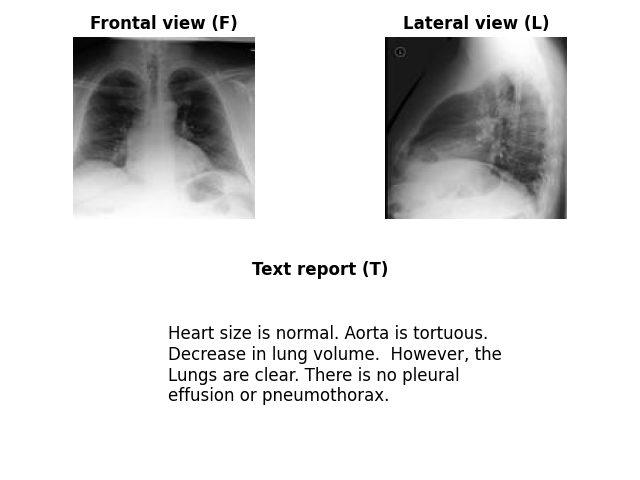
\includegraphics[width=0.6\textwidth]{data/rand_dataset_sample.png}
        \end{figure}

    \end{frame}

    \begin{frame}{The Labels}
        \pause
        \begin{itemize}
            \item Because the labels are highly unbalanced, we created a binary label "Finding".
            \begin{itemize}
                \item If sample presents any pathology $\rightarrow$ finding = True, else False
            \end{itemize}
            \item This results in 14529 samples that are annotated with the "Finding" label in the training set and 47218 samples that are not.
        \end{itemize}
    \end{frame}

    \begin{frame}{The word Encoding}

        \small{
            "Heart size is normal." $\rightarrow [0,1,2,3] \rightarrow$ Model $\rightarrow
            \begin{bsmallmatrix}
                1 & 0 & 0 & 0\\
                0 & 1 & 0 & 0\\
                0 & 0 & 1 & 0\\
                0 & 0 & 0 & 1\\
            \end{bsmallmatrix}$
            $\rightarrow [0,1,2,3] \rightarrow$ "Heart size is normal."}\\
        \vspace{\baselineskip}
        \pause
        \begin{itemize}
            \item Every word that occurs at least 3 times in all the text reports is mapped to an index.
            \pause
            \item Using this mapping each sentence is encoded into a sequence of indices.
            \pause
            \item The output of the decoder is in a one-hot-encoded format.
        \end{itemize}
    \end{frame}

    \subsection{The model architecture}
    \begin{frame}{The model}
        \begin{itemize}
            \item The MoPoE-VAE has an independent encoder and decoder for each modality (F, L and T).
            \item In this work we used a ResNet \footcite{he2016deep} type architecture for all encoders and decoders.
        \end{itemize}

    \end{frame}

    \subsection{Evaluation methods}

    \begin{frame}{Evaluation Methods}
        \begin{itemize}
            \item Evaluation of the separability of the latent representation
            \item Evaluation of the generation coherence
        \end{itemize}
    \end{frame}

    \begin{frame}{Evaluation of the latent representation}
        \begin{figure}[!h]
            \centering
            \begin{tikzpicture}

                \begin{scope}[blend group = soft light]
                    \fill[blue!40!white]   (0:0) ellipse (6cm and 2.9cm);
                    \fill[green!40!white] (0:-2) ellipse (1.5cm and 2cm);
                    \fill[red!40!white]  (0:2) ellipse (1.5cm and 2cm);
                    \draw [-,ultra thick] (0,-1.5) -- (0,1.5);
                \end{scope}
                \node at (0:-2)   {"No Finding"};
                \node at (0:2)   {"Finding"};
                \node at (90:2.3) [font=\Large] {Latent Representation};
                \node at (-90:1.8) [font=\tiny] {Linear Classifier};
            \end{tikzpicture}
        \end{figure}

    \end{frame}

    \begin{frame}{Evaluation of the latent representation}
        \begin{figure}[!h]
            \centering
            \begin{tikzpicture}
                \begin{scope}[blend group = soft light]
                    \fill[blue!40!white]   (0:0) ellipse (6cm and 2.9cm);
                    \fill[green!40!white] (0:-1) ellipse (3cm and 2cm);
                    \fill[red!40!white]  (0:1) ellipse (3cm and 2cm);
                \end{scope}
                \node at (0:-2)   {"No Finding"};
                \node at (0:2)   {"Finding"};
                \node at (90:2.3) [font=\Large] {Latent Representation};
            \end{tikzpicture}
        \end{figure}
    \end{frame}

    \begin{frame}{Evaluation of the generation coherence}
        \begin{itemize}
            \item The generated samples are classified using trained ResNet \footcite{he2016deep} classifiers.
            \pause
            \item If the modalities of a sample, generated and given as conditioner, are classified as having the same label, they are considered coherent.
        \end{itemize}


    \end{frame}

    \subsection{Hyper-Parameter Selection}
    \begin{frame}{Hyper-Parameter Selection}
        %We used a simple grid search to find the best hyperparameters, retaining the parameter values that resulted in the best performance on the evaluation of the latent representation.\\
        %Namely, a value of 1 for the $\beta$ parameter and a \hyperlink{mopoe_graph}{\textit{class dimension}} of 512 gave the best separability of the latent space.
        \begin{center}
            \begin{table}[]

                \begin{tabular}{ c c c }
                    Parameter                                         & Best         & Search Space                \\
                    \midrule
                    $\beta$\footnote{\textbf{Loss:} $\sum_m^{\#mods} w_m \cdot log\_prob_m + \beta \cdot joint\_divergence $}
                    & \textbf{1.0}
                    & [0.001, 0.01, 0.5, 1.0, 5, 20]
                    \\
                    \hyperlink{mopoe_graph}{\textit{class dimension}} & \textbf{512} & [32, 64, 96, 128, 256, 512] \\
                    Img Size                                          & \textbf{128} & [64, 128, 256]
                \end{tabular}
                %\caption{\textbf{Table showing the results of the parameter grid search.}}
            \end{table}

        \end{center}

    \end{frame}


    \section{Results}

    \subsection{Evaluation of the Latent Representation}

    \begin{frame}{Mean AP for the MoPoE}
        \begin{table}
            \centering
            \begin{tabular}{llrrrrrrr}
                MODEL & LABEL   & F     & L     & T     & L,F   & F,T   & L,T   & L,F,T          \\
                \midrule
                MoPoE & Finding & 0.706 & 0.679 & 0.776 & 0.684 & 0.790 & 0.785 & \textbf{0.804} \\

            \end{tabular}
            \caption{\textbf{Classification results of the linear classifiers trained on the learned latent representation using the binary label "Finding". The mean average precision over the test set
            is reported for each modality (F: frontal image, L: lateral image, T: text report).}}
        \end{table}
        \pause
        \small{\textbf{Note}: The frontal view is the most informative view for chest X-rays, according to radiologists (\cite{kovaleva2020towards}).}
    \end{frame}

%    \begin{frame}{Mean AP for the MoPoE}
%        \py{
%            pytex_tab(
%            script='scripts/lr_table_bin.py',
%            label='lr_table_bin',
%            caption='\\textbf{Classification results of the linear classifiers trained on the learned latent representation using the binary label "Finding". The mean average precision over the test set
%            is reported for each modality (F: frontal image, L: lateral image, T: text report).}',
%            options_post='',
%            )
%        }
%        \pause
%        \small{\textbf{Note}: The frontal view is the most informative view for chest X-rays, according to radiologists (\cite{kovaleva2020towards}).}
%    \end{frame}

    \begin{frame}{Comparison with the ResNet classifiers}
        \begin{table}
            \centering
            \begin{tabular}{llrrrrrrr}
                MODEL & LABEL   & F     & L     & T     & L,F  & F,T            & L,T   & L,F,T \\
                \midrule
                MoPoE & Finding & 0.706 & 0.679 & 0.776 & 0.684 & 0.790 & 0.785 & \textbf{0.804} \\

            \end{tabular}
            \caption{\textbf{Classification results of the linear classifiers trained on the learned latent representation.}}
        \end{table}

        \py{
            pytex_tab(
            script='scripts/clf_table_bin.py',
            caption='\\textbf{Classification results for the ResNet classifiers.}',
            options_post='',
            )
        }
    \end{frame}

%    \begin{frame}{Comparison with the ResNet classifiers}
%        \py{
%            pytex_tab(
%            script='scripts/lr_table_bin.py',
%            caption='\\textbf{Classification results of the linear classifiers trained on the learned latent representation.}',
%            options_post='',
%            )
%        }
%
%        \py{
%            pytex_tab(
%            script='scripts/clf_table_bin.py',
%            caption='\\textbf{Mean AP values for the supervised classifiers.}',
%            options_post='',
%            )
%        }
%    \end{frame}

    \subsection{Generation Evaluation}

    \begin{frame}
        \begin{table}[]
            \centering
            \begin{tabular}{lcccccccccc}

                & & \multicolumn{3}{c}{F} & \multicolumn{3}{c}{L,F} & \multicolumn{3}{c}{L,F,T} \\  \cmidrule(l){3-5} \cmidrule(l){6-8} \cmidrule(l){9-11} MODEL & LABEL & F & L & T & F & L & T & F & L & T \\\midrule
                MoPoE & Finding & 0.547 & 0.501 & 0.492 & 0.563 & 0.515 & 0.505 & \textbf{0.569} & 0.519 & 0.534
            \end{tabular}
            \caption{\small{\textbf{Evaluation of the generation coherence.} For conditional generation, the letter below the horizontal line indicates the modality which is generated based on the input subsets $\xset _k$ above. We report the mean average precision values between the prediction of a trained classifier on the generated samples and the label of the input samples.}}
        \end{table}
        \pause
        The random baseline lies at \py{boilerplate.print_rand_perf()}.

    \end{frame}

    \begin{frame}{Conditionally generated samples with L and T modalities as conditioner.}

        \begin{figure}
            \centering
            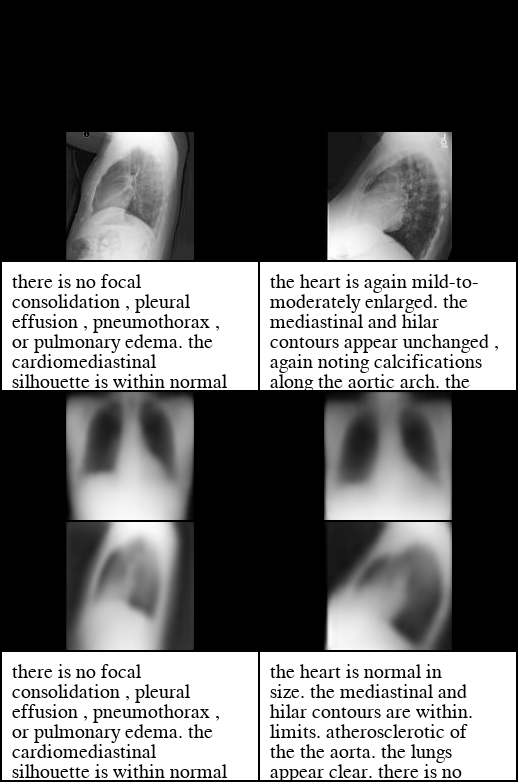
\includegraphics[width=0.6\textwidth, height = 0.85\textheight, keepaspectratio]{slides/cond_gen/Lateral_text_blacked.png}

        \end{figure}
    \end{frame}

    \begin{frame}{Adding the F modality as conditioner}
        \begin{figure}
            \centering
            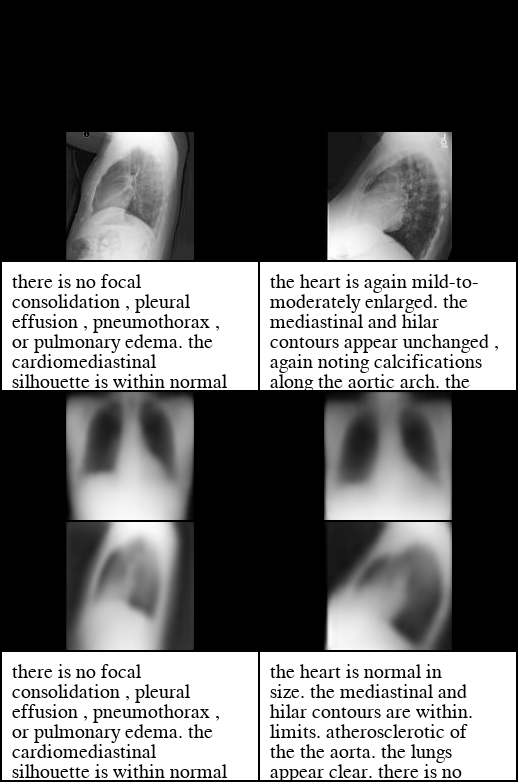
\includegraphics[width=0.6\textwidth, height = 0.85\textheight, keepaspectratio]{slides/cond_gen/Lateral_text_blacked.png}
            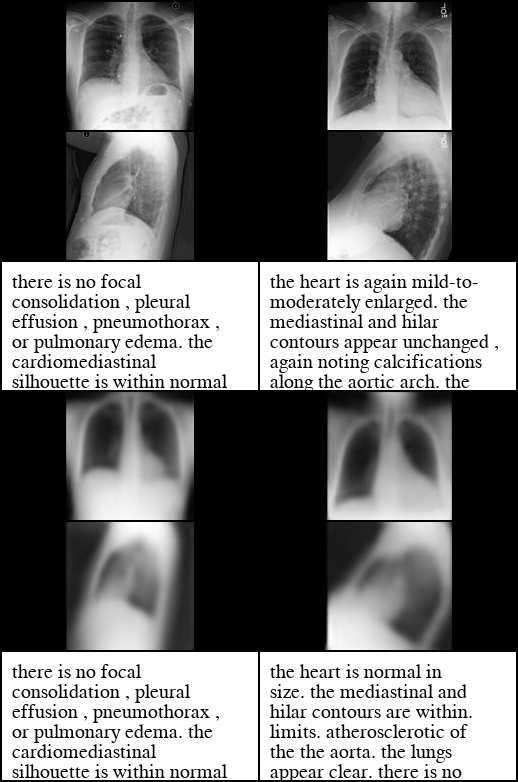
\includegraphics[width=0.6\textwidth, height = 0.85\textheight, keepaspectratio]{slides/cond_gen/Lateral_PA_text.png}
        \end{figure}
    \end{frame}

    \begin{frame}{The model struggles to generate the T modality when it is not given}
        \begin{figure}
            \centering
            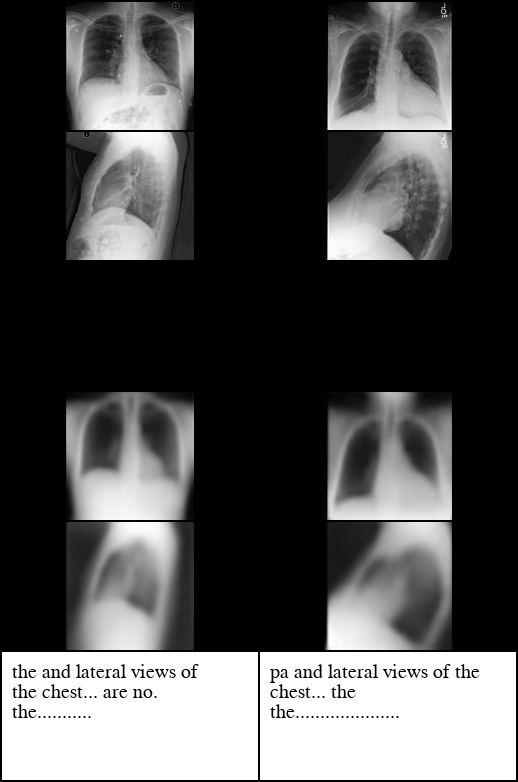
\includegraphics[width=0.6\textwidth, height = 0.85\textheight, keepaspectratio]{slides/cond_gen/Lateral_PA_small_censored.png}
            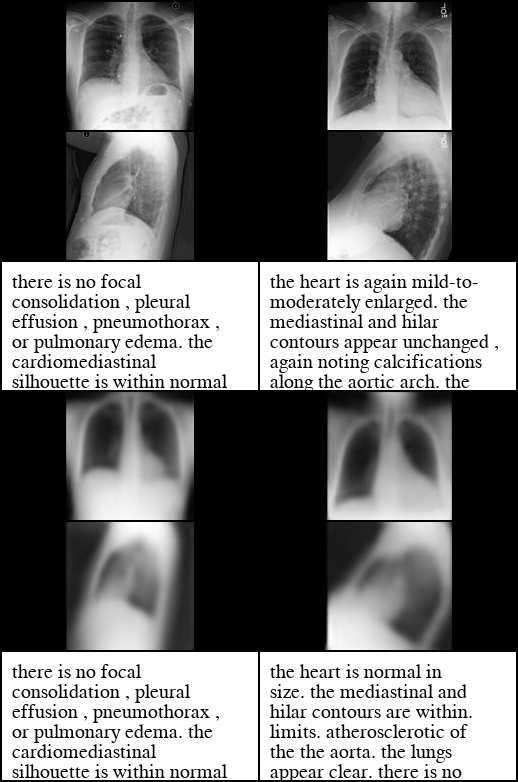
\includegraphics[width=0.6\textwidth, height = 0.85\textheight, keepaspectratio]{slides/cond_gen/Lateral_PA_text.png}
        \end{figure}
    \end{frame}


    \section{Conclusion}
    \begin{frame}{Conclusion}
        We showed that:
        \begin{itemize}
            \item The MoPoE method provides promising results when applied to medical data for:
            \begin{itemize}
                \item Classification
                \item Generation
            \end{itemize}
            \item However, we also highlighted some problems that can still be addressed to improve the performance.
        \end{itemize}
    \end{frame}

    \begin{frame}{Future Work}
        \begin{itemize}
            \item Finding better architecture for the decoder and encoder parts.
            \item Finding a better prior than the Gaussian distribution. \footcite{zhao2017towards}
            \item Trying state-of-the-art method such as
            \begin{itemize}
                \item Vector Quantised-Variational AutoEncoder \footcite{oord2018neural}
                \item Deep Hierarchical Variational AutoEncoder \footcite{vahdat2021nvae}
            \end{itemize}

        \end{itemize}

    \end{frame}

    \printbibliography


    \section{Supplementary}

    \begin{frame}{Resnet}
        Residual Neural Networks are a popular architecture for deep learning models.
        Since its publication in an article from \cite{he2016deep}, it has been widely used (cited over 70453 times) for image recognition tasks.
        \begin{figure}
            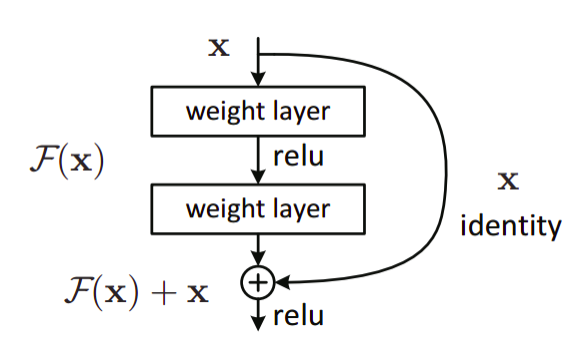
\includegraphics[width=0.3\textwidth, keepaspectratio]{slides/Residual_block}
            \caption{Residual learning: a building block. Taken from \cite{he2016deep}.}
        \end{figure}
    \end{frame}

    \begin{frame}
        \begin{figure}
            \centering
            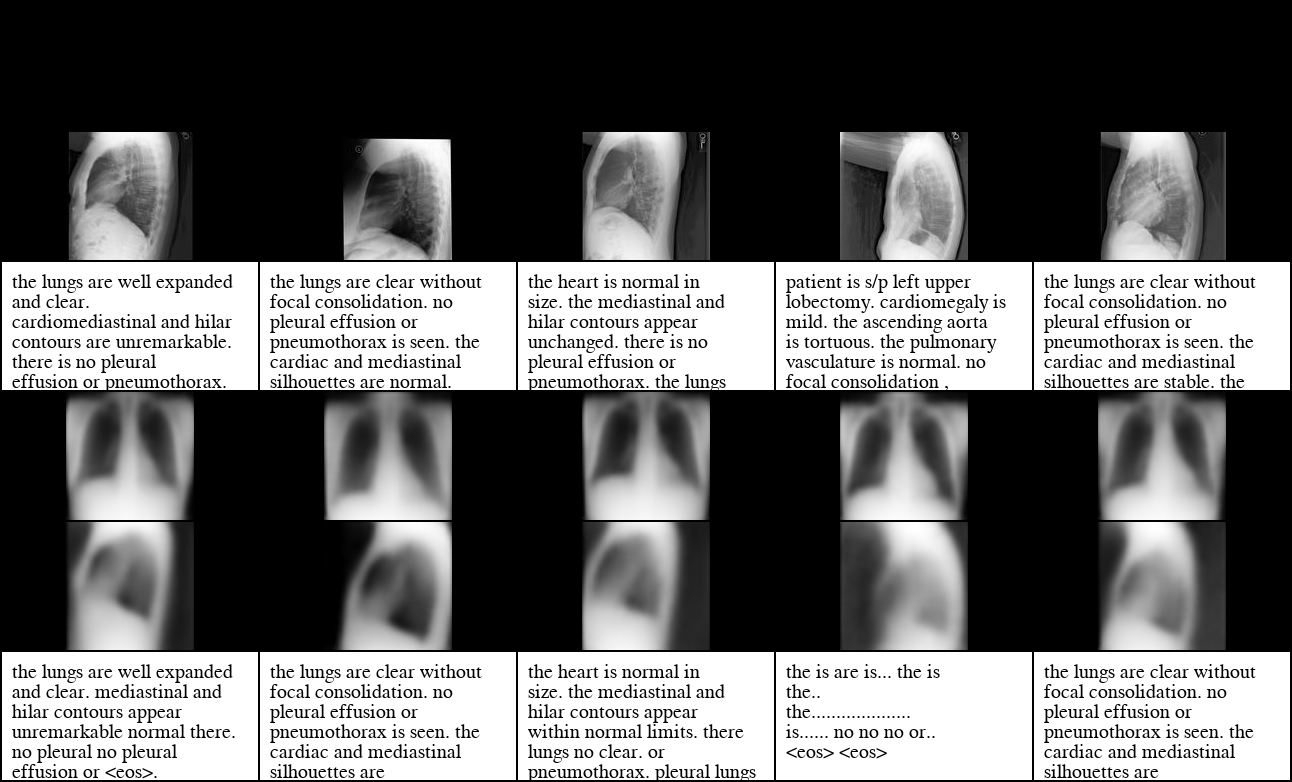
\includegraphics[width=0.6\textwidth, height = \textheight, keepaspectratio]{data/cond_gen/Lateral_text_censored}
            \caption{\tiny{
                \textbf{Conditionally generated samples with F and T modalities as conditioner.} The second and third image rows were given to the model as conditioner. The three last images rows are the generated samples. The images in the first row are the radiographs that correspond to the samples given as conditioner. The generated samples are blurry and it is difficult to see whether they represent some of the features that are characteristic to the input samples.
            }}
        \end{figure}
    \end{frame}

    \begin{frame}
        \begin{figure}
            \centering
            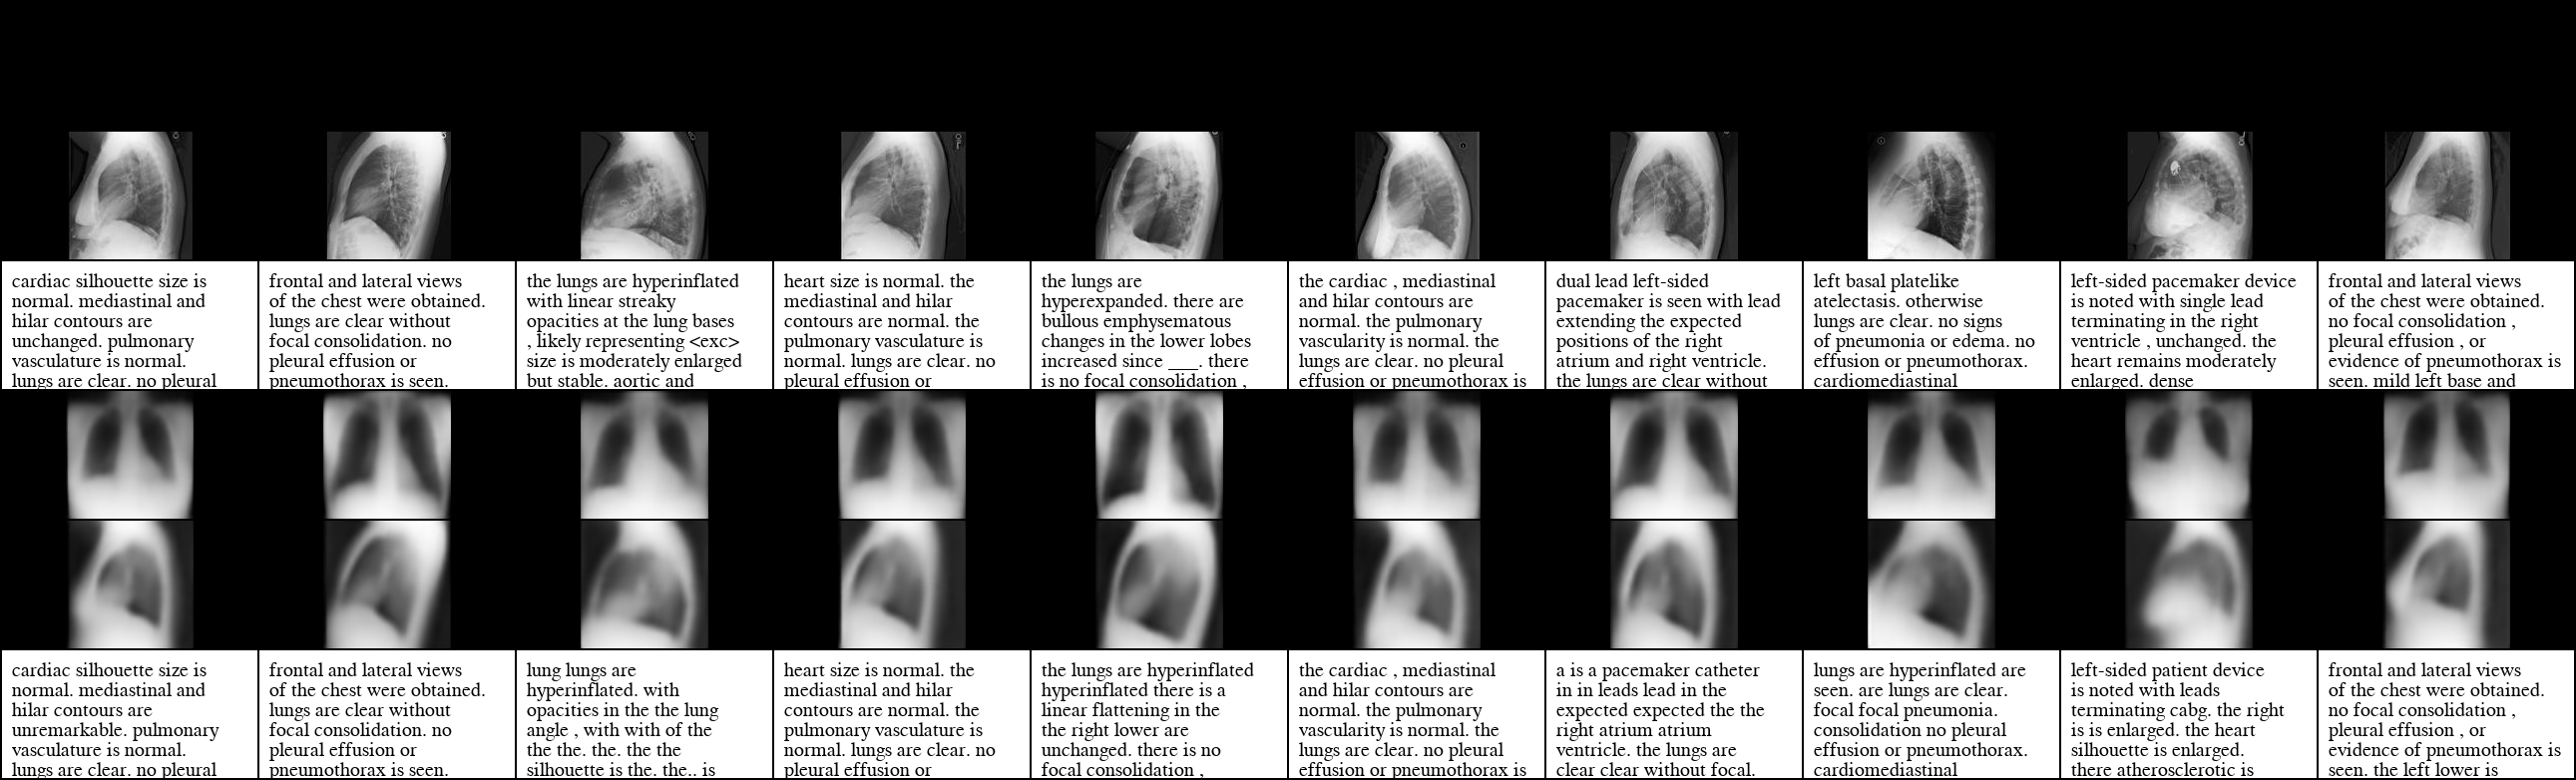
\includegraphics[width=0.6\textwidth, height = \textheight, keepaspectratio]{data/cond_gen/Lateral_text}
            \caption{\tiny{
                \textbf{Conditionally generated samples with F and T modalities as conditioner.} The second and third image rows were given to the model as conditioner. The three last images rows are the generated samples. The images in the first row are the radiographs that correspond to the samples given as conditioner. The generated samples are blurry and it is difficult to see whether they represent some of the features that are characteristic to the input samples.
            }}
        \end{figure}
    \end{frame}


    \begin{frame}
        \begin{figure}
            \centering
            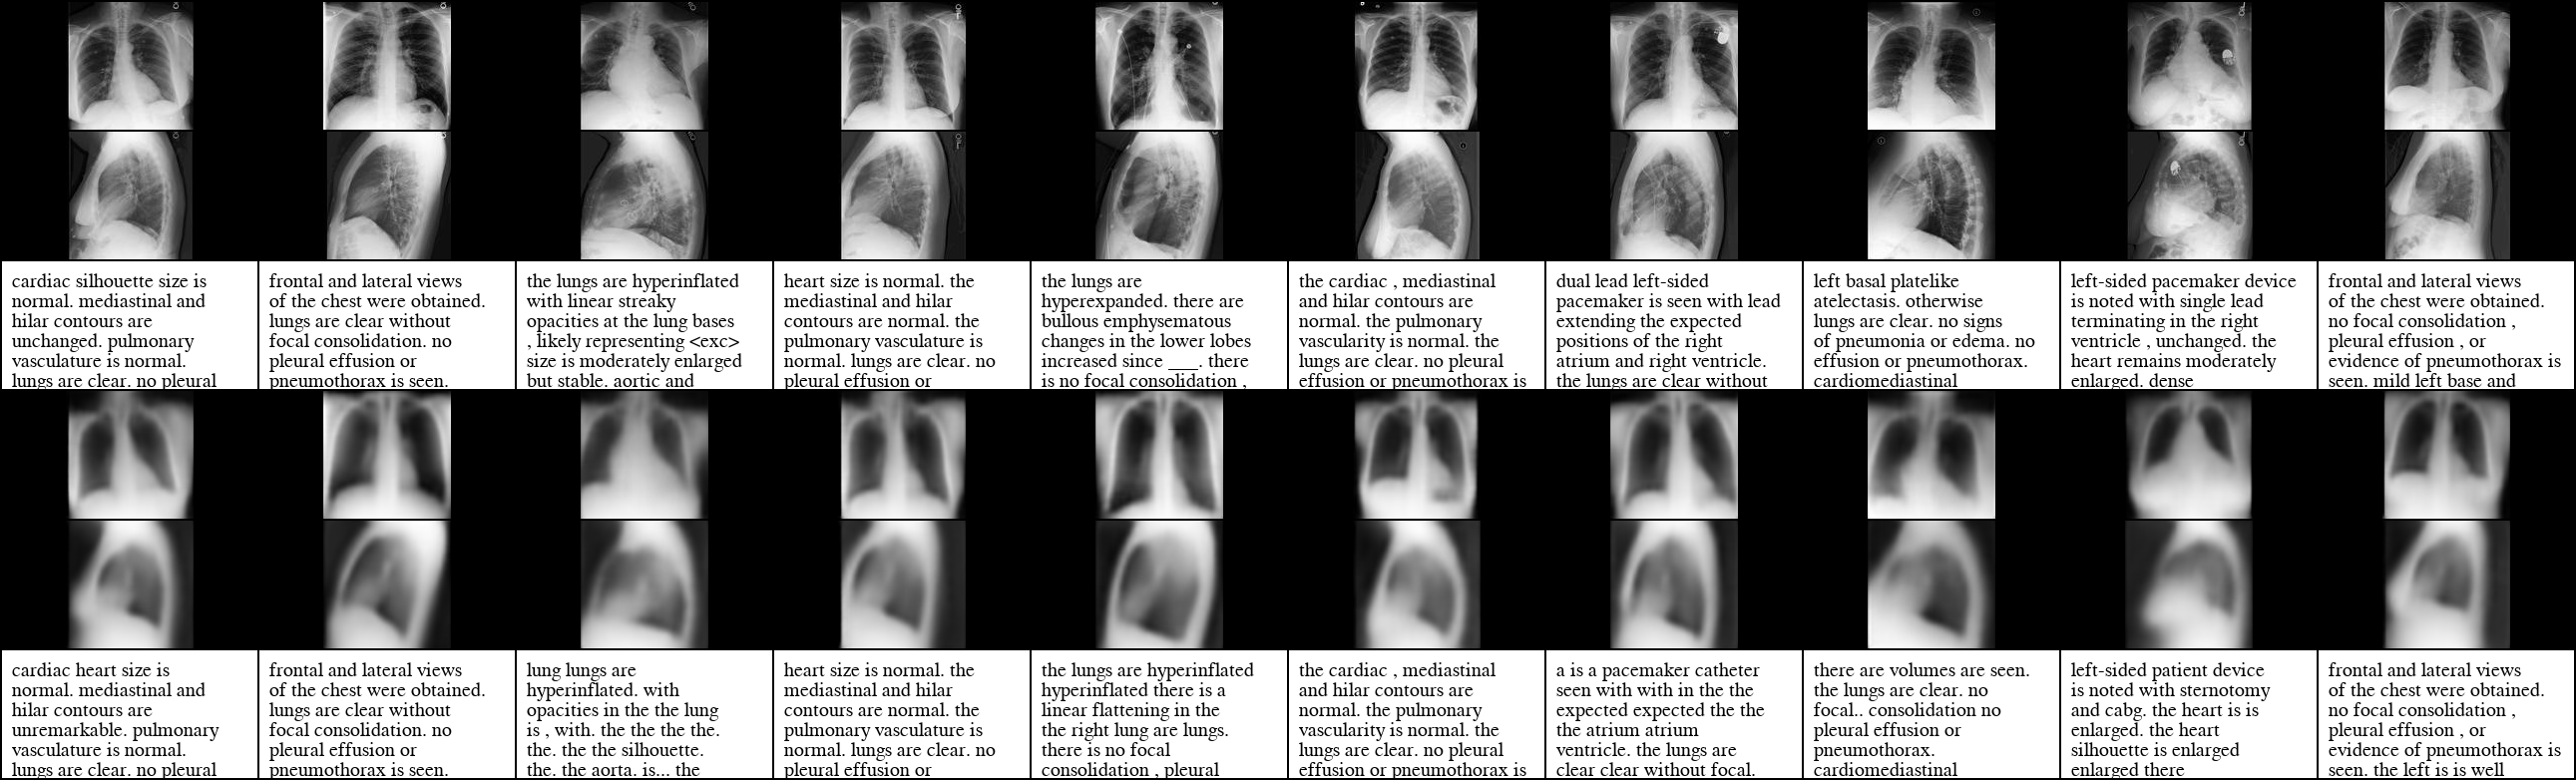
\includegraphics[width=0.6\textwidth, height = \textheight, keepaspectratio]{data/cond_gen/Lateral_PA_text}
            \caption{\textbf{Conditionally generated samples with F, L and T modalities as conditioner.}}
        \end{figure}
    \end{frame}

    \begin{frame}{The PoE-VAE}

        \begin{itemize}
            \item Uses a geometric mean: the joint posterior is a product of individual posteriors
            %p(z|x_1,...,x_N)) \propto p(z) \prod _{i=1} ^N \tilde{q}(z|x_i)
            \begin{equation}
                q_{\Phi}(z|x_{1:M})=\prod _m q_{\Phi_m}(z|x_m)
            \end{equation}
            \item Results in a good approximation of the joint distribution but struggles in optimizing the individual experts.
            \item If one of the expert is miscalibrated (bad initialisation, overconfidence), it will perturb the whole joint distribution.
        \end{itemize}
    \end{frame}

    \begin{frame}{The MoE-VAE}
        \begin{itemize}
            \item Uses an arithmetic mean: the joint posterior is a sum of individual posteriors
            \begin{equation}
                q_{\Phi}(z|x_{1:M})=\sum _m \alpha_m\cdot q_{\Phi_m}(z|x_m)
            \end{equation}
            \item Optimizes individual experts well but is not able to learn a distribution that is sharper than any of its experts.
        \end{itemize}

    \end{frame}


    \begin{frame}
        \py{
            pytex_tab(
            script='scripts/clf_table_allmetrics.py',
            caption='\\textbf{Metric values for the supervised classifiers.}',
            options_post='',
            )
        }
    \end{frame}

    \begin{frame}
        \py{
            pytex_tab(
            script='scripts/lr_table_allmetrics.py',
            caption='\\textbf{Metric values for the supervised classifiers.}',
            options_post='',
            )
        }
    \end{frame}

\end{document}
